\documentclass[crop,tikz,border=0,convert=pdf2svg,multi=false]{standalone}
\usepackage[T1]{fontenc}
\usepackage{amsfonts}
\usepackage[defaultsans]{opensans}
\usetikzlibrary{shapes,matrix,arrows,positioning}
\begin{document}
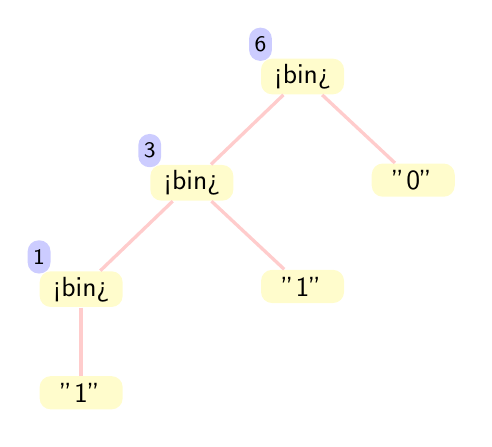
\begin{tikzpicture}[font=\sffamily,
  mymat/.style = {
    matrix of nodes, row sep=2.5em, column sep=1em, nodes=mynode},
  mynode/.style = {
    fill=yellow!20, rectangle, rounded corners, inner sep=.2em, minimum
    height=1.2em, minimum width=3em}]

  \matrix (m) [mymat] {
    & & <bin> & \\
    & <bin> & & "0" \\
    <bin> & & "1" & \\
    "1" & & & \\
  };

  \begin{scope}[red!20,very thick]
    \draw (m-1-3) -- (m-2-2);
    \draw (m-1-3) -- (m-2-4);
    \draw (m-2-2) -- (m-3-1);
    \draw (m-2-2) -- (m-3-3);
    \draw (m-3-1) -- (m-4-1);
  \end{scope}

  \begin{scope}[every node/.style={font=\footnotesize\sffamily,fill=blue!20, rectangle, rounded
      corners, inner sep=.2em, minimum height=1.2em}]
    \foreach \i/\j/\k in {1/3/6,2/2/3/,3/1/1} {
      \node at ([yshift=0.5em]m-\i-\j.north west) {\k}; }
  \end{scope}

\end{tikzpicture}
\end{document}
